\documentclass[12pt]{article}
\usepackage[utf8]{inputenc}
\usepackage{graphicx} % Per includere immagini
\usepackage{titling}  % Per personalizzare lo spazio del titolo
\usepackage{ccicons}  % Per i simboli Creative Commons
\usepackage{geometry} % Per personalizzare i margini
\usepackage{hyperref} % Per i link
\usepackage[italian]{babel}
\usepackage{pgffor}
\usepackage{listings}
\usepackage{color}
\usepackage{float}
\usepackage{pdflscape}


\definecolor{codegreen}{rgb}{0,0.6,0}
\definecolor{codegray}{rgb}{0.5,0.5,0.5}
\definecolor{codepurple}{rgb}{0.58,0,0.82}
\definecolor{backcolour}{rgb}{0.95,0.95,0.92}

\lstdefinestyle{mystyle}{
    backgroundcolor=\color{backcolour},   
    commentstyle=\color{codegreen},
    keywordstyle=\color{magenta},
    numberstyle=\tiny\color{codegray},
    stringstyle=\color{codepurple},
    basicstyle=\ttfamily\footnotesize,
    breakatwhitespace=false,         
    breaklines=true,                 
    captionpos=b,                    
    keepspaces=true,                 
    numbers=left,                    
    numbersep=5pt,                  
    showspaces=false,                
    showstringspaces=false,
    showtabs=false,                  
    tabsize=2
}

\lstset{style=mystyle}

% Imposta i margini della pagina
\geometry{
  top=2cm,
  bottom=2cm,
  left=3cm,
  right=3cm
}

\lstset{
  basicstyle=\ttfamily,
  breaklines=true,
  columns=fullflexible
}

\setlength{\droptitle}{-5em} % Sposta in alto il titolo

\title{
    \Large \textbf{UNIVERSITA' DI SALERNO} \\[0.5em]
    \small DIPARTIMENTO DI INGEGNERIA DELL'INFORMAZIONE ED ELETTRICA E MATEMATICA APPLICATA\\[5em]
    
\includegraphics[width=0.6\textwidth]{logo_uni.png}\\[3em] % Logo dell'Università
    \normalsize Laurea Magistrale in Ingegneria Informatica \\[1em]
    \Large \textbf {Project work} \\[1em]
    \large \textbf {Deliverable 2} \\ [1em]
    \large {Sistemi Embedded} \\[1em]
}

\author{
    \textbf{Gruppo: 8} \\
    \normalsize Marotta Giuseppe - 0622702302 - g.marotta31@studenti.unisa.it\\
    \normalsize Rea Gaetano - 0622702190 - g.rea7@studenti.unisa.it\\
    \normalsize Squitieri Giuseppe - 0622702339 - g.squitieri8@studenti.unisa.it\\ 
    \normalsize Tramice Davide - 0622702194 - d.tramice@studenti.unisa.it\\ \\
    }

\date{
    ANNO ACCADEMICO 2023/2024 % Data
}

\begin{document}

\begin{titlingpage} % Crea una pagina di titolo personalizzata
\maketitle
\thispagestyle{empty} % Rimuove il numero di pagina
%\begin{center}
    %\ccbyncnd % Simbolo Creative Commons
%\end{center}
\end{titlingpage}

% Creazione di una nuova pagina
\newpage


% Aggiungi l'indice delle sezioni
\tableofcontents


\newpage


\section{Implementazione}

In accordo con la progettazione descritta nel capitolo precedente, in questo capitolo verrà dettagliata l'implementazione del modello Stateflow. Si inizierà con una panoramica generale, per poi scendere progressivamente a livelli di dettaglio sempre maggiori.

\section{Descrizione del Modello}

Il modello Stateflow è stato sviluppato per gestire i vari stati e le transizioni del sistema di controllo del cancello automatico. I principali componenti del modello includono:

\begin{itemize}
    \item \textbf{Sistema di Controllo del Cancello}: Gestisce gli stati di apertura, chiusura, controllo dei tempi e gestione degli ostacoli.
    \item \textbf{Pulsanti di Controllo}: Include i pulsanti B1, B2 e B3 per l'apertura/chiusura, la regolazione del tempo di chiusura e la regolazione del tempo di lavoro, rispettivamente.
    \item \textbf{Sensori di Ostacolo}: Sensori P1 e P2 per rilevare la presenza di ostacoli e per il controllo sulla chiusura completa del cancello.
    \item \textbf{Indicatori LED}: LED verde, giallo e rosso per indicare lo stato del cancello (aperto, chiuso, in movimento, errore).
\end{itemize}

\begin{figure}[H]
    \centering
    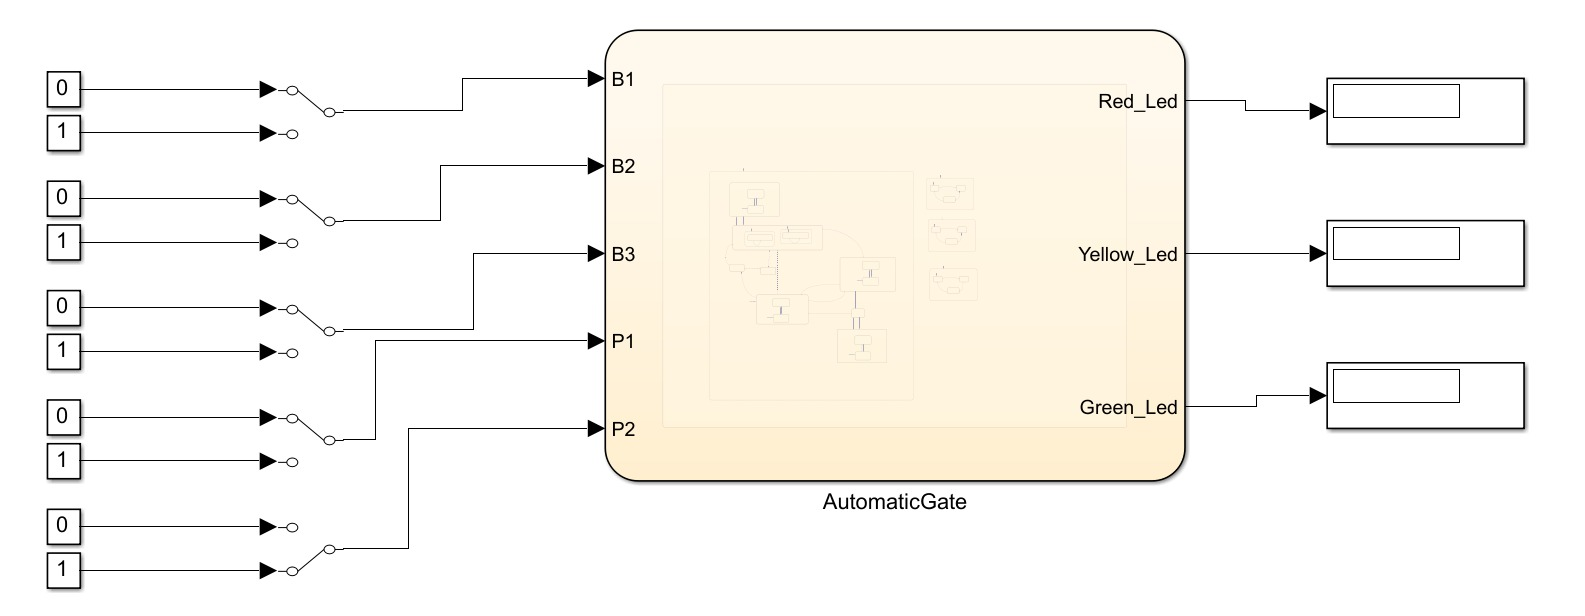
\includegraphics[width=1\textwidth]{Immagini_State_Flow/Vista_Generale.jpg}
    \caption{Vista Generale del Sistema.}
\end{figure}

\section{Introduzione al Core del Cancello}

Nel core del nostro sistema, troviamo vari stati che lavorano in parallelo: \textbf{Automatic Gate, B1, B2, B3}. Lo stato \textbf{Automatic Gate} gestisce tutta la logica di funzionamento del cancello, mentre gli altri stati gestiscono la corretta pressione dei rispettivi pulsanti.

\subsection{Pulsante B1}

Descriviamo nel dettaglio lo stato del pulsante B1. Questo componente viene utilizzato per richiedere l'apertura o la chiusura del cancello e sono previsti tre super-stati: \textbf{RELEASED, PRESSED, LONGPRESSED}.

\begin{enumerate}
    \item \textbf{RELEASED}: Stato iniziale. Si passa allo stato \textbf{PRESSED} quando viene rilevata la pressione del pulsante B1.
    \item \textbf{PRESSED}: Stato attivo durante la pressione del pulsante. Se viene rilevato un fronte di discesa, si passa allo stato \textbf{LONGPRESSED}.
    \item \textbf{LONGPRESSED}: Stato transitorio che, quasi istantaneamente, ritorna allo stato di \textbf{RELEASED}. Prima di tornare allo stato di \textbf{RELEASED}, viene eseguita un'azione che indica l'evento "B1\_pressed".
\end{enumerate}

Successivamente, descriveremo come questo evento impatta sulla logica di funzionamento nello stato \textbf{AUTOMATIC GATE}.

\begin{figure}[H]
    \centering
    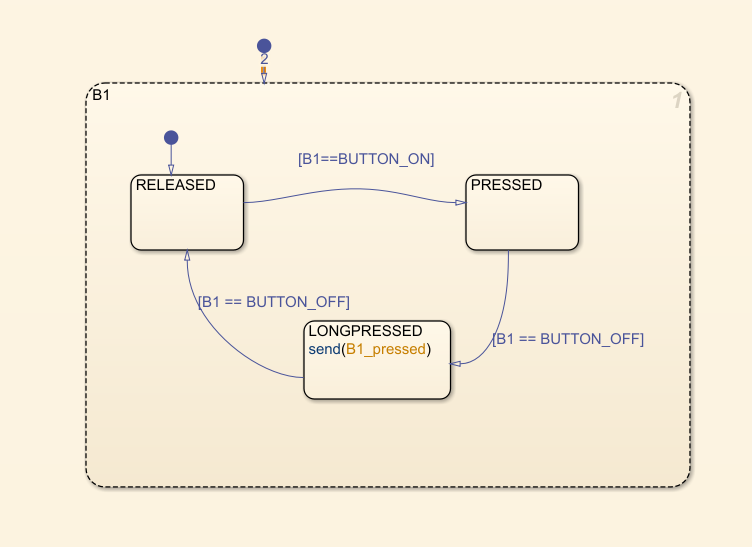
\includegraphics[width=1\textwidth]{Immagini_State_Flow/Pulsante_B1.png}
    \caption{Pulsante B1.}
\end{figure}

\subsection{Pulsante B2 e B3}

Il Pulsante B2 è utile per regolare il tempo di chiusura automatica del cancello, mentre il pulsante B3 è usato per il settaggio dei valori del Tempo di Lavoro in fase di apertura e chiusura. Entrambi condividono lo stesso funzionamento del Pulsante B1 descritto precedentemente.

\begin{figure}[H]
    \centering
    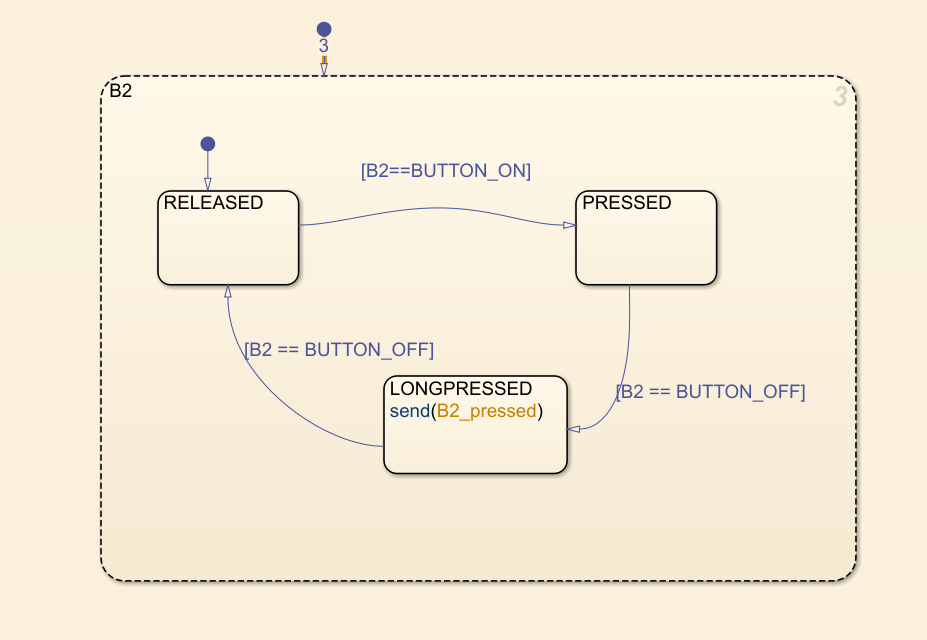
\includegraphics[width=1\textwidth]{Immagini_State_Flow/Pulsante_B2.png}
    \caption{Pulsante B2.}
\end{figure}

\begin{figure}[H]
    \centering
    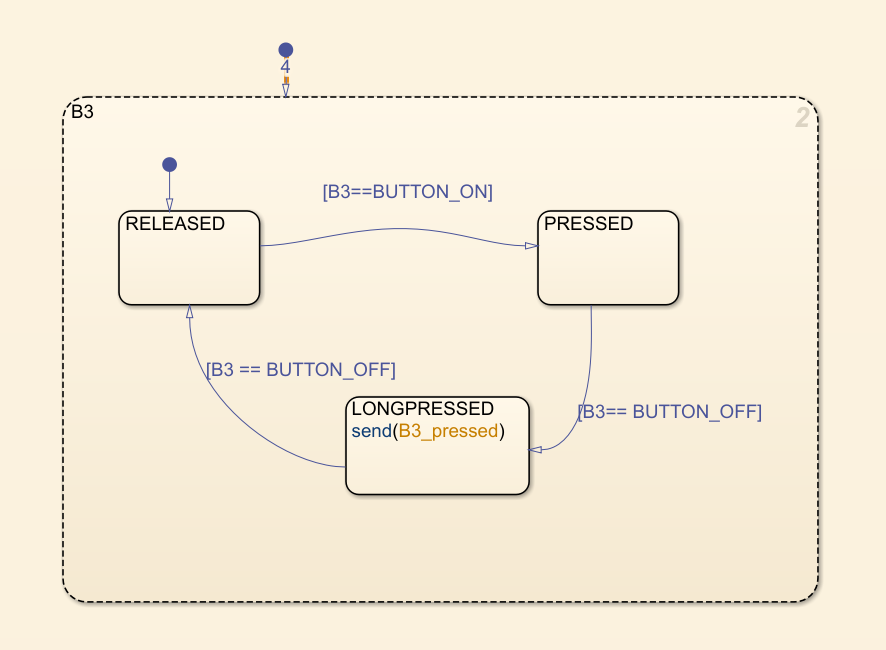
\includegraphics[width=1\textwidth]{Immagini_State_Flow/Pulsante_B3.png}
    \caption{Pulsante B3.}
\end{figure}

\subsection{Automatic Gate}

Arriviamo ora a descrivere lo stato che implementa la logica di funzionamento. Innanzitutto, come scelta implementativa, consideriamo come Stato Iniziale lo stato \textbf{CLOSING}. Consideriamo quest'ultimo tale poiché le specifiche richiedono che al momento dell'attivazione del sistema, se il cancello è aperto, ovvero P2 è inattivo, quest'ultimo passi in uno stato di chiusura descritto appunto dal suddetto stato. All'interno troviamo due super-stati \textbf{YELLOW\_ON} e \textbf{YELLOW\_OFF} che descrivono il Toggle del LED Giallo che avviene con frequenza 0.5 Hz.

\begin{figure}[H]
    \centering
    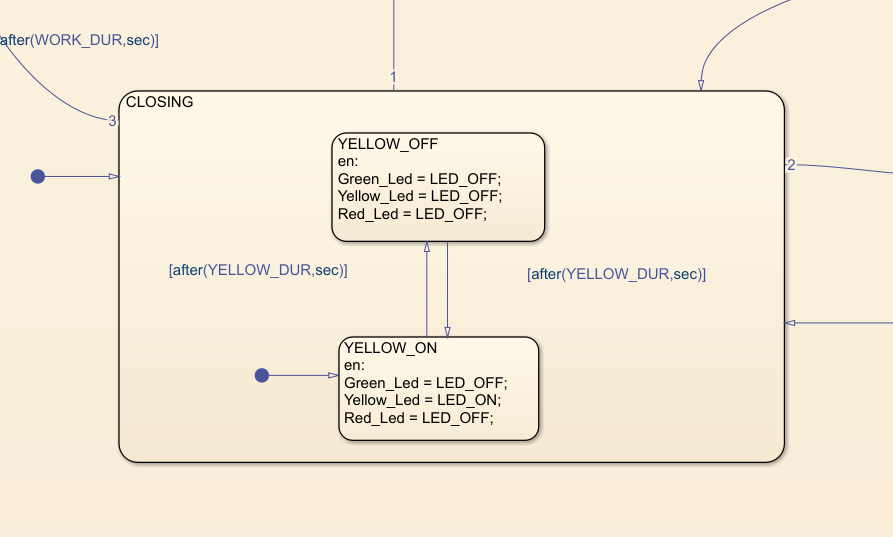
\includegraphics[width=1\textwidth]{Immagini_State_Flow/Closing.png}
    \caption{Closing State.}
\end{figure}

Nel momento in cui il cancello si chiude completamente o è già chiuso (P2 è attivo), si passa allo stato \textbf{CLOSED}. In questo stato, tutti i LED sono spenti e al suo interno troviamo due super-stati: \textbf{OPEN\_DUR\_SETTING} e \textbf{WORK\_DUR\_SETTING} che descrivono il settaggio dei parametri del tempo di chiusura automatica e del tempo di lavoro, che può essere attuato solo se il sistema si trova in questo stato. Per descrivere questi stati interni prenderemo in esame \textbf{OPEN\_DUR\_SETTING}, poiché il discorso è analogo per \textbf{WORK\_DUR\_SETTING}. Quando viene premuto B2, viene generato un evento che poi viene catturato da quest'ultimo stato e viene effettuata un'operazione che modifica la variabile \textbf{OPEN\_DUR}: 

\[
\textit{OPEN\_DUR} = \textit{mod((OPEN\_DUR), 120) + 10}
\]

Questo perché i valori impostati hanno un range (10, 120).

\begin{figure}[H]
    \centering
    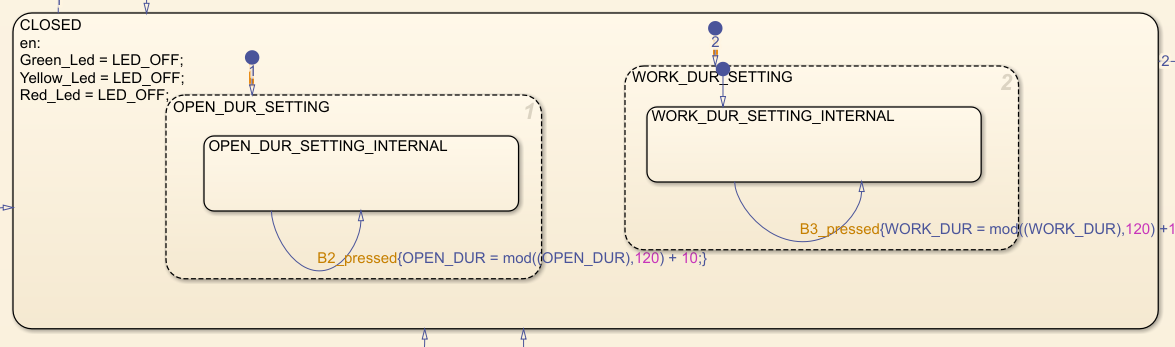
\includegraphics[width=1\textwidth]{Immagini_State_Flow/Closed.png}
    \caption{Closed State.}
\end{figure}

Chiaramente dallo stato di \textbf{CLOSED} si passa a \textbf{OPENING} nel momento in cui viene premuto B1. Al suo interno troviamo il Toggling del LED Giallo con lo stesso meccanismo di \textbf{CLOSING}.

\begin{figure}[H]
    \centering
    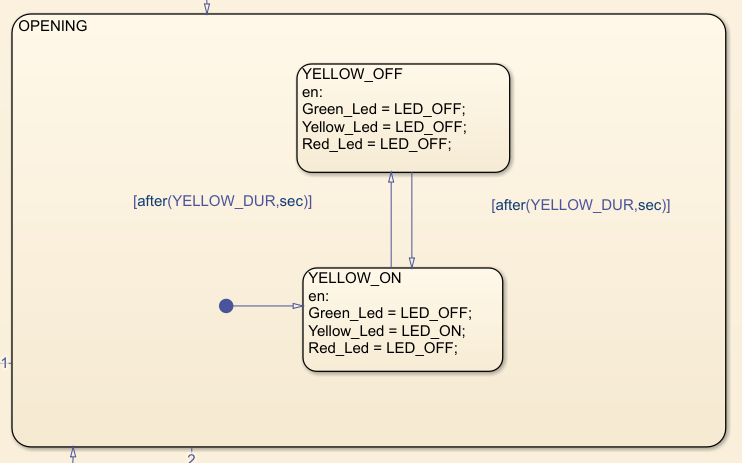
\includegraphics[width=1\textwidth]{Immagini_State_Flow/Opening.png}
    \caption{Opening State.}
\end{figure}

Appena finito il tempo di lavoro, il cancello va nello stato \textbf{OPEN} dove tutti i LED sono accesi.

\begin{figure}[H]
    \centering
    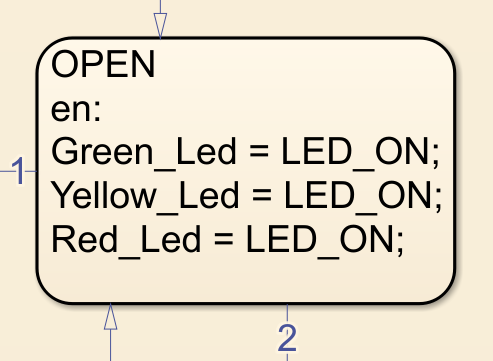
\includegraphics[width=1\textwidth]{Immagini_State_Flow/Open.png}
    \caption{Open State.}
\end{figure}

\subsection{Emergency States}

Dallo stato \textbf{OPEN}, per tornare di nuovo in uno stato di chiusura, è possibile premere il pulsante B1 o attendere la chiusura automatica. Tuttavia, come specificato, il cancello non eseguirà il comando di chiusura se il sensore P1 è attivo, ma passerà nello stato \textbf{EMERGENCY\_P1\_OPEN}. Il sistema rimane in questo stato per 30 secondi o finché il sensore P1 non ritorna inattivo. Al suo interno troviamo due super-stati che descrivono il toggling del LED verde: \textbf{GREEN\_ON} e \textbf{GREEN\_OFF} con frequenza 1 Hz.

\begin{figure}[H]
    \centering
    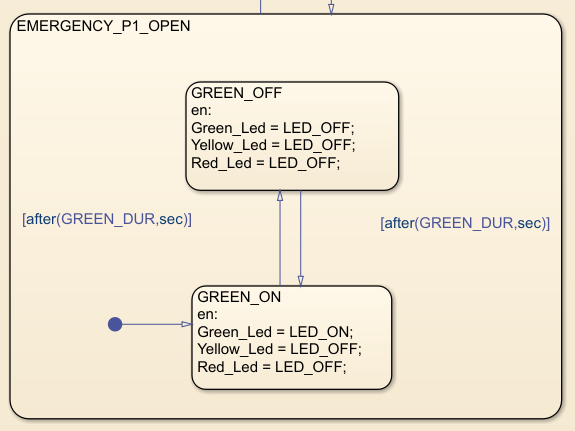
\includegraphics[width=1\textwidth]{Immagini_State_Flow/Emergency_P1_Open.png}
    \caption{Emergency P1 Open State.}
\end{figure}

Se P1 è attivo quando il cancello è chiuso e viene premuto il pulsante B1, il sistema passerà in uno stato analogo: \textbf{EMERGENCY\_P1\_CLOSED}.

\begin{figure}[H]
    \centering
    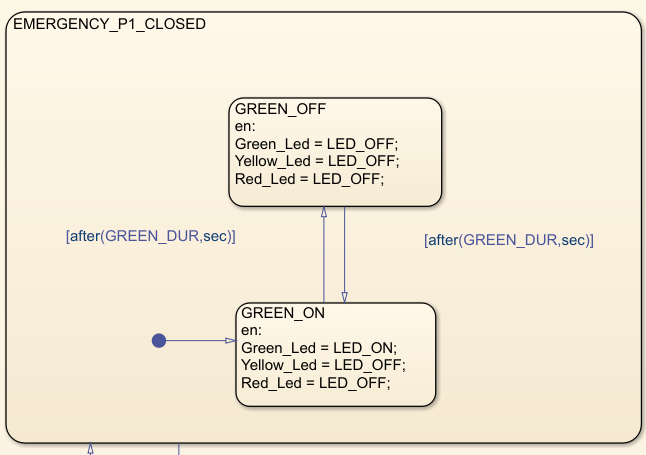
\includegraphics[width=1\textwidth]{Immagini_State_Flow/Emergency_P1_Closed.png}
    \caption{Emergency P1 Closed State.}
\end{figure}

Infine, descriviamo due stati che indicano una situazione di emergenza più grave (vero e proprio malfunzionamento del sistema): \textbf{EMERGENCY} e \textbf{EMERGENCY\_LED}. Lo stato \textbf{CLOSING} può durare al massimo un tempo T di lavoro, oltrepassato il quale, se P2 non è attivo, il sistema va in un primo stato \textbf{EMERGENCY} dove tutti i LED sono spenti e rimane per 10 secondi. Trascorsi questi 10 secondi, se P2 non è attivo, il sistema passa nello stato \textbf{EMERGENCY\_LED} dove è attivo il LED di emergenza rosso.

\begin{figure}[H]
    \centering
    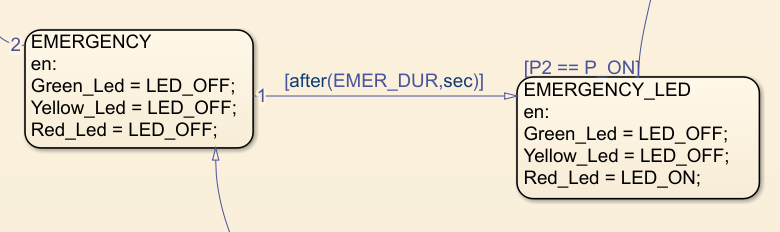
\includegraphics[width=1\textwidth]{Immagini_State_Flow/Emergency.png}
    \caption{Emergency State.}
\end{figure}

\end{document}